\chapter{Dataset and Preprocessing}

For this thesis, data from two different sources was collected and processed: the \textit{Perverted Justice} (PJ) archive and the \textbf{PAN12} Sexual Predator Identification dataset.

\section{PAN12 Dataset}
The PAN12 Sexual Predator Identification Corpus was introduced by Inches and Crestani as part of CLEF 2012 and represents the first large-scale benchmark dataset for the automatic detection of sexual predators in chat conversations~\cite{inches2012pan}. The PAN12 dataset was designed for two specific tasks: First, identifying sexual predators among all users, and second, detecting specific chat lines that are most characteristic of predatory behavior. It remains a reference benchmark in cyber grooming detection and has been employed in a lot of follow-up studies~\cite{inches2012pan}.

The collection combines four distinct sources: 

\begin{enumerate}
    \item Perverted Justice logs containing confirmed grooming conversations
    \item Omegle chats between consenting adults
    \item IRC logs from \textit{irclog.org}
    \item IRC logs from \textit{krijnhoetmer.nl}
\end{enumerate}

 This composition was chosen to include both genuine positive cases and potentially misleading negative examples containing sexual explicit but non-grooming messages.  

The dataset comprises a total of \textbf{357{,}622 conversations}.  
Among them:  
\begin{itemize}
    \item \textbf{11{,}350 conversations (\approx 3.17\%)} originate from \textit{Perverted Justice (PJ)} logs and constitute the \textbf{positive class (grooming)}.
    \item \textbf{346{,}272 conversations} represent the \textbf{negative class}.
\end{itemize}

The data was split in the following way.

\begin{itemize}
    \item \textbf{Training set:}
    \begin{itemize}
        \item 66{,}927 conversations
        \item 903{,}607 messages
        \item 97{,}689 unique authors, including 142 predators
    \end{itemize}
    \item \textbf{Test set:}
    \begin{itemize}
        \item 155{,}128 conversations
        \item 2{,}058{,}781 messages
        \item 218{,}702 unique authors, including 254 predators
    \end{itemize}
\end{itemize}

And can be seen as a classification task of either a binary classification between predator and non-predator chats. Also, the conversation can be classificated in thre different ways, with a distinction of:

\begin{itemize}
    \item \textbf{(P)} Grooming conversations
    \item \textbf{(A)} Sexual conversations between adults
    \item \textbf{(N)} Non-sexual chats
\end{itemize}

A big challenge of the Pan12 dataset is the \textbf{class imbalance}, as only a small fraction of all conversations are grooming-related, making the detection of sexual predators and relevant text passages particularly difficult.

%% geändert

\section{Perverted Justice (PJ) Dataset}
The Perverted Justice (PJ) dataset~\cite{pj} is based on chat logs collected by the U.S.-based Perverted Justice Foundation, which undertook a proactive approach in the detection of online sexual predators. They trained adult volunteers posed as young people (decoy victims) in chat rooms and engaged in conversations with adults who have sexual intentions towards minors and to record these interactions. The goal was to identify and report potential predators to law enforcement agencies. Once the adult was convicted in an American Court of Law, the Foundation made all the material related to them available online for public access. The PJ dataset consists of chat logs from over 600 confirmed grooming cases, with each conversation containing multiple messages. The conversations are typically structured as dialogues between a decoy victim and an adult groomer. PJ data has been used in nearly all major peer-reviewed studies on automatic grooming detection and form the basis for the positive class in the PAN12 dataset.~\cite{inches2012pan} 
The organisation ended its operations in 2019 following public criticism because of the controversial nature of its methods and the potential risks to decoy victims. Therefore, the original PJ dataset is no longer publicly available. However, archived chat logs remain available upon request for research purposes.~\cite{pj}

\subsection{Data Acquisition and Integration Strategy}

For this thesis, in order to increase the size and completeness of the cybergrooming class, it was decided to scrape the Perverted Justice (PJ) archive and integrate the data with the negative samples of PAN12, since it already contains a subset of all PJ conversations. This made sure that all available PJ data was used, while also benefiting from the additional non-grooming conversations in PAN12.

\subsubsection{Collecting Perverted Justice (PJ) Data}

Following a formal request, academic access to an archived version of the site via the Internet Archive (Wayback Machine) was granted. Based on this permission, the full archive was retrieved and processed for research purposes.

A custom scraping tool was developed to extract all available chat logs from a 2023 snapshot. Chat dialogues were extracted from the HTML structure by identifying \textit{<div class="chatLog">} sections and splitting them into lines. Regular expressions were used to clean the data, removing timestamps, HTML comments, and formatting artifacts. 

After scraping, the pipeline proceeded as follows:
\begin{itemize}
    \item \textbf{Scraping:} All chat logs were downloaded and extracted. This resulted in \textbf{605} raw PJ chat sessions which consisted of several partial conversations over a long period of time.
    \item \textbf{Parsing:} Speaker-message pairs were extracted using regex rules and normalized. Conversations were split into multiple sub-dialogues whenever empty lines indicated a topic or session change. This yielded \textbf{10,811} parsed PJ chat sessions across all extracted files.
    \item \textbf{Anonymization:} A batch-wise anonymization step was applied to ensure privacy and remove personally identifiable information. This included replacing emails with \textit{[EMAIL]}, URLs with \textit{[URL]}, IP addresses with \textit{[IP]}, and phone numbers with \textit{[PHONE]}.
    \item \textbf{Filtering:} Conversation Sessions with fewer than 8 messages were removed, resulting in \textbf{6,175} grooming-labeled conversations.
    \item \textbf{Final preprocessing:} The remaining chats were standardized into a uniform JSON format with labeled roles (groomer/decoy), consistent dialogue structure, and metadata fields.
\end{itemize}

The final PJ grooming dataset consists of \textbf{6,175} labeled conversations.

\subsubsection{Adding PAN12 Data (Non-Grooming Subset)}
To create a reliable negative class, a filtered subset of the PAN12 dataset was used. PAN12 contains over 100{,}000 conversations, including more than 5{,}000 involving known sexual predators. Still, many PAN12 chats are really short, consisting of only 1-2 messagess. The preprocessing steps were as follows:

\begin{itemize}
    \item \textbf{Raw corpus loading:} The full dataset consists of \textbf{66,927} training and \textbf{155,128} test conversations, totaling \textbf{222,055} chats across both splits.
    \item \textbf{Initial filtering:} All conversations involving identified predators or labeled as containing grooming behavior (according to the official PAN12 ground truth) were excluded, since they were already included in the PJ dataset.
    \item \textbf{Participant \& length constraints:} Only conversations with exactly two participants and a minimum of 8 messages were kept.
    \item \textbf{Spam removal \& quality filtering:} An additional manual filtering step excluded problematic cases:
    \begin{itemize}
        \item Extremely short, non-linguistic messages (for example \enquote{m}, \enquote{e}, \enquote{?\_?}).
        \item Symbolic or spam-like ASCII sequences (for example \enquote{yearyearyear\ldots} or repeated \enquote{WARNING} messages).
        \item Excessively long sequences that could not be meaningfully tokenized or chunked (for example single messages with over 512 tokens).
    \end{itemize}
\end{itemize}

For the PAN12 dataset, anonymization was already conducted during dataset creation. As stated by Inches and Giacomo~\cite{inches2012pan}, all personal identifiers (for example names, emails, phone numbers, URLs) were removed or replaced by synthetic placeholders prior to release. After all preprocessing and filtering steps, the resulting PAN12 non-grooming dataset contained \textbf{27,755} full conversations.

All further preprocessing steps were applied across both datasets and integrated into the pipeline prior to modeling.

\section{Slang and Informal Language Handling}

For preprocessing the chat data, a script was developed that uses the OpenAI API (\textit{gpt-4.1-mini}) to perform slang normalization. The employed prompt specified the following rules:
\begin{enumerate}
    \item \textbf{Replace slang, internet abbreviations, and leetspeak} (for example \textit{wanna} $\rightarrow$ ``want to'', \textit{ur} $\rightarrow$ ``you'') with their standard English equivalents.
    \item \textbf{Resolve predefined placeholders} according to a mapping table (for example \textit{\_\_laugh\_\_} $\rightarrow$ ``haha'', \textit{\_\_thinking\_\_} $\rightarrow$ ``hmm'').
    \item \textbf{Correct obvious spelling and grammar mistakes}.
    \item \textbf{Do not modify} emojis, emoticons, or stylistic punctuation sequences (for example \textit{:P}, \textit{XD}, \textit{??}).
    \item \textbf{Preserve} the informal style and emotional tone, including explicit or manipulative language.
\end{enumerate}

This normalization was performed \emph{prior} to fine-tuning BERT for the following three key reasons:

\subsubsection{Avoiding source effects}  
The dataset combines conversations from different sources (PAN12 and PJ). Without normalization, the model could exploit differences in slang usage as a shortcut, instead of learning actual grooming-related patterns. Therefore, it might be the case that it is too easy for the model to learn the decision boundary for these two classes, not because the model is good at detecting sexual predators, but because these two datasets were generated in different ways~\cite{schlaepfer2022online}.

\subsubsection{Synchronizing BERT and LIWC input}  
The planned model fusion relies on BERT embeddings and LIWC features extracted from the \emph{same} text chunks. BERT processed the raw text while LIWC analyzed the cleaned text, a semantic mismatch would occur~\cite{he2021deberta}. Consistency ensures that, for example:  
\textit{``This chunk had high LIWC values in the sexuality category and was also classified as grooming by BERT.''}
 
\subsubsection{Improving model efficiency and robustness}  
Uniformly cleaned text results in more stable tokenization, reduces rare tokens, avoids model misinterpretations, and can improve performance by removing noise~\cite{sun-etal-2023-tokenization}.

Additionally, LIWC relies on a fixed dictionary and does not recognize misspelled words~\cite{pennebaker2022liwc}. Without correction, such words would not be assigned to any category, leading to incomplete feature counts. Normalization ensures, that relevant terms are correctly mapped to their LIWC categories and a more accurate LIWC analysis can be performed.

\section{Raw Conversational Length Distributions }

\begin{figure}[H]
    \centering
    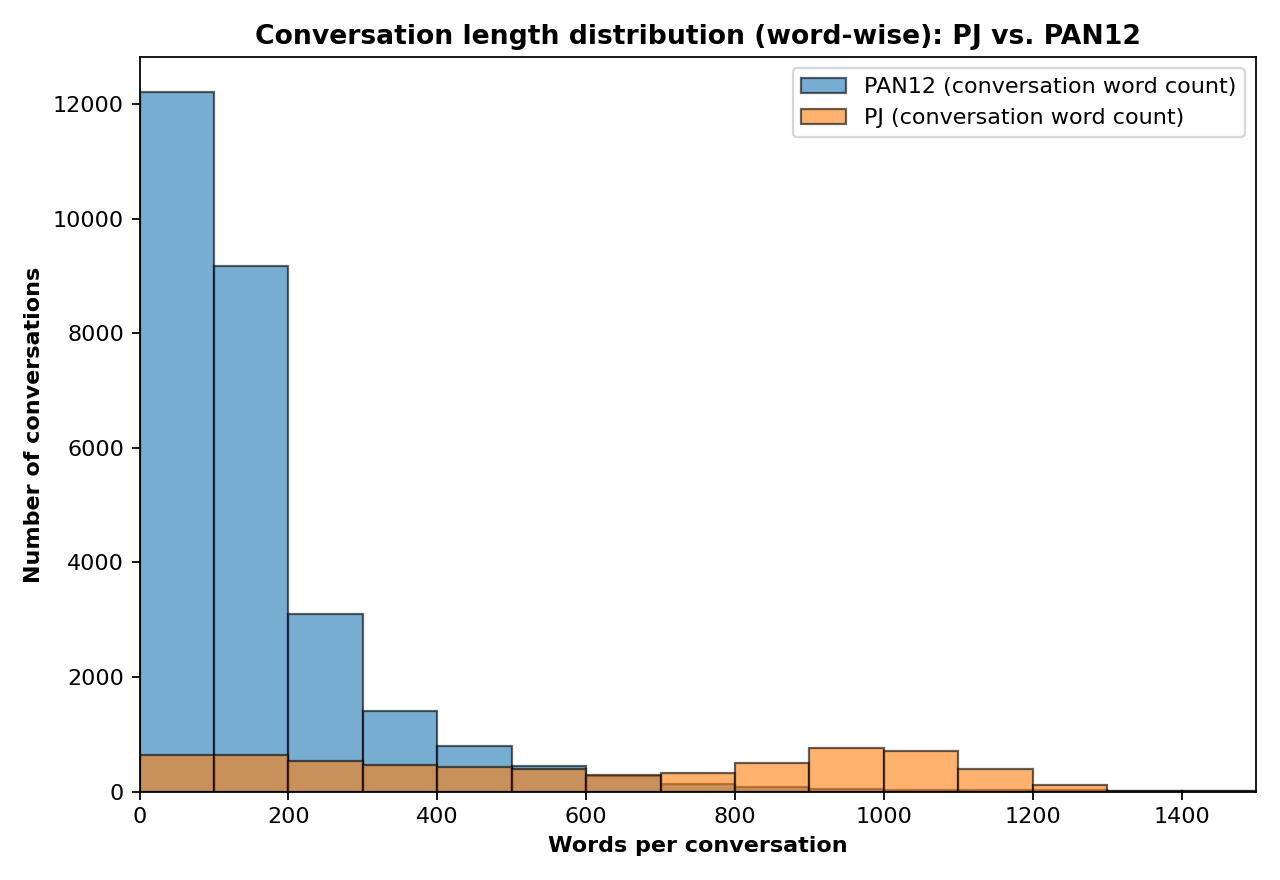
\includegraphics[width=0.75\textwidth]{conversation_word_lengths_pj_vs_pan12.png}
    \caption[Raw Conversational Length Distributions]{Comparison of raw conversational length distributions (in words) between PJ and PAN12 datasets.}
    \label{fig:conversation_word_lengths}
\end{figure}

After initial preprocessing, the length distributions of the raw conversations in both datasets were analyzed. Figure~\ref{fig:conversation_word_lengths} shows the number of words per conversation for both PJ and PAN12 datasets. It is apparent, that PJ conversations are clearly longer than those from PAN12. This difference in length is a potential confounder, as the model could exploit it as a shortcut for classification instead of learning semantic patterns. Therefore, the preprocessing pipeline was designed to reduce this effect by enforcing fixed-length chunking and incorporating synthetic non-grooming data in PJ style.


\section{Generating Synthetic Non-Grooming Data}\label{sec:synthetic-data}

To further increase model robustness and mitigate dataset-specific artifacts, a custom script was developed that  uses the OpenAI API (\textit{gpt-4.1-mini}) to generate synthetic negative examples in the style of the Perverted Justice (PJ) data. The employed prompt contained the following rules:
\begin{enumerate}
\item \textbf{Replicate the linguistic style of PJ chats} by providing the model with 100 already normalized PJ conversations as few-shot examples.
\item \textbf{Enforce strict formatting}, requiring every line to follow the pattern \textit{speaker\_1: \textless text \textgreater} or \textit{speaker\_2: \textless text \textgreater}.
\item \textbf{Generate long dialogues} with 90–120 turns, in order to reduce the risk of length-based shortcuts. This choice was made because PJ conversations are usually much longer than those from PAN12 (see Figure \ref{fig:conversation_word_lengths} for a comparison of conversation length distributions).
\item \textbf{Restrict content} to everyday, harmless topics without any references to sexual activity.
\item \textbf{Include small imperfections} (for example occasional double dots, lowercase starts, or short fragments) to match the PJ normalization profile more closely, while keeping the conversations coherent.
\end{enumerate}

The synthetic data generation was done for the following two main purposes:

\begin{itemize}
    \item \textbf{Avoiding length leakage:} By generating long synthetic non-grooming conversations in PJ style, the data balance is improved and the reliance on length as a shortcut is reduced.
    \item \textbf{Avoiding domain leakage:} Since all PJ chats are labeled as class 0 and all PAN12 chats as class 1, the model could learn to separate classes only based on dataset-specific style differences. The synthetic PJ-style non-grooming data helps to reduce this effect by providing negative examples that mirror the PJ distribution without grooming semantics.
\end{itemize}

Unfortunately it was not possible to generate synthetic grooming conversations in the PAN12 style due to usage restrictions. Therefore, only non-grooming chats were created, ensuring that no artificial grooming data was introduced.


\section{Final Dataset}

The final dataset used for model training and evaluation consists of the following grooming and non-grooming conversations from the three sources: PJ, PAN12, and synthetic data. The final conversation counts are the following:

\begin{itemize}
    \item \textbf{PJ: 6175 Dialogues}
    \item \textbf{PAN12: 27755 Dialogues}
    \item \textbf{Synthetic: 600 Dialogues with mean lenght of 150 messages}
\end{itemize}


%%%geändert





